
%(BEGIN_QUESTION)
% Copyright 2009, Tony R. Kuphaldt, released under the Creative Commons Attribution License (v 1.0)
% This means you may do almost anything with this work of mine, so long as you give me proper credit

Determine the correct potentiometer millivoltage settings to generate the following temperature indications at the instrument:

$$\includegraphics[width=15.5cm]{i02976x01.eps}$$

\begin{itemize}
\item{} -93$^{o}$ F ; Potentiometer setting = \underbar{\hskip 50pt} mV 
\vskip 5pt
\item{} 157$^{o}$ F ; Potentiometer setting = \underbar{\hskip 50pt} mV 
\vskip 5pt
\item{} 389$^{o}$ F ; Potentiometer setting = \underbar{\hskip 50pt} mV  
\vskip 5pt
\item{} 580$^{o}$ F ; Potentiometer setting = \underbar{\hskip 50pt} mV  
\end{itemize}

\underbar{file i02976}
%(END_QUESTION)





%(BEGIN_ANSWER)

\begin{itemize}
\item{} -93$^{o}$ F ; Potentiometer setting = \underbar{\bf -4.540} mV 
\item{} 157$^{o}$ F ; Potentiometer setting = \underbar{\bf 2.400} mV 
\item{} 389$^{o}$ F ; Potentiometer setting = \underbar{\bf 9.466} mV  
\item{} 580$^{o}$ F ; Potentiometer setting = \underbar{\bf 15.353} mV  
\end{itemize}

%(END_ANSWER)





%(BEGIN_NOTES)


%INDEX% Measurement, temperature: thermocouple

%(END_NOTES)


